\documentclass[11pt, a4paper]{article}
\usepackage{graphicx}
\usepackage{amsmath, bm}
\usepackage{natbib}
\usepackage[utf8]{inputenc}    
\usepackage{natbib}
\usepackage[usenames,dvipsnames]{xcolor}
\usepackage[left=2cm,right=2cm,top=2cm,bottom=2cm]{geometry}
\usepackage{hyperref}
\usepackage[outdir=./]{epstopdf}
\usepackage{lscape}
\usepackage{multirow}
\usepackage{booktabs} % Create TABS
\usepackage{array,arydshln}  % CREATE DASH LINE
\title{Identification of stably expressed genes in RNA-Seq data of  Arabidopsis}
\date{} % Today's date or a custom date


\begin{document}
\maketitle

\section*{Abstract}
We examined RNA-Seq data on 165 biological samples from 18 different
experiments carried out by different labs and identified genes that are stably
expressed across biological samples, experiment conditions, and labs. We fit a
random-effect model to the read counts for each gene and decompose the total
variance to into between-sample, between-condition and between-lab variance
components. Identifying stably expressed genes is useful for count
normalization. The variance component analysis is a first step towards
understanding the sources and nature of the RNA-Seq count variation.


\section{Introduction}

\textbf{Why is normalization important}
RNA sequencing (RNA-Seq) has become the technology of choice for transcriptome
profiling over the last few years. A key task of RNA-Seq analysis is to detect
differentially expressed (DE) genes under various experimental or
environmental conditions. Count normalization are needed for adjusting
differences in sequencing depths or library sizes (total numbers of mapped
reads for each biological sample) due to chance variation in sample
preparation.  In DE analysis, gene expression levels are often estimated from
relative read frequencies. For this reason, normalization is also needed to
account for the apparent reduction or increase in relative read frequencies of
non-differentially expressing genes simply to accommodate the increased or
decreased relative read frequencies of truly differentially expressing genes.

\textbf{Why is stably expressed gene important}
A central idea to many existing count normalization methods is to identify and
use as reference a set of stably expressed genes whose expression levels are
known or expected to not vary much under different experimental conditions.
For example, the trimmed mean of M-values normalization method	(TMM) \citep{robinson2010scaling} and DESeq normalization \citep{anders2010differential}  assume that the majority of
the genes are not DE within an experiment. 
Implicitly, these methods use genes with relatively small observed fold
changes under a single experiment as a reference gene set in normalization.
There are two obvious issues with this strategy: 1. The available sample size
in any single experiment may be too small for us to reliably estimate true
fold changes. 2.  If the experiment condition can affect expression levels of
more than half of the genes (\cite{loven2012revisiting}, \cite{wu2013use}), many of the existing normalization methods may be unreliable. 

\textbf{How to find stably expressed genes}
In microarray studies, the so-called "housekeeping genes" (HKGs) are often
used as reference genes for normalization. HKGs are typically constitutive
genes that maintain basic cellular function, and therefore are expected to
express at relatively constant levels in non-pathological situations.
However, many studies have shown that HKGs are not necessarily stably
expressed (a review can be found in \cite{huggett2005real} and reference therein). 
For example, in the microarray analysis of classical model plant
\textit{Arabidopsis thaliana} (Arabidopsis), \cite{czechowski2005genome}
showed that traditional HKGs such as ACT2, TUB6, EF-1$\alpha$ are not
stably expressed, and thus not good reference genes for normalization.  
A similar idea is to use spike-in genes, but \cite{risso2014nat} showed that spike-in genes are not necessarily stably
expressed and thus may not help normalization. HKGs or spike-in genes are therefore not a given prior for reference genes, and careful evaluation should be performed when they are being used in normalization.


\textbf{Numerically finding stably expressed genes.}
% Why would we bother to study them under RNA-Seq since there are related works in microarray} (some sentense are needed to connect the two paragraphs)
Another quite successful approach to identify stably expressed genes is through screening a large number of microarray data sets. Typically, large sets of microarry data are compiled for a given experimental condition, and stably expressed genes are validated and recommended for potential use.  In general, validation experiments show that these genes are better than traditional HKGs. By investigating 721 arrays of 323 conditions throughout development, \cite{czechowski2005genome} suggested reference genes for a variety of experimental series for Arabidopsis. \cite{stamova2009identification} collected 526 samples of human blood  data and validated a subset of most stably expressed genes they identified. Similar studies were carried out for Arabidopsis seed\citep{dekkers2012identification}, breast tumor tissues[cite], mouse (universal)[cite] and so on. 

\textbf{What is our goal and the approach} 
 We implemented generalized linear mixed model (GLMM) \citep{mccullagh1989generalized} to examine stably expressed genes for Arabidopsis RNA-Seq data. RNA-Seq is superior to microarray technology because of its high-throughput, pricise measurement, as well as sensitivity for gene expressed at both low and very high levels \citep{wang2009rna}. The exponential growth in RNA-Seq study accumulates a large amount of Arabidopsis
data under a variety of experimental/enviromental conditions. It is therefore possible to evaluate stably expressed genes with RNA-Seq data. The aim of this study is twofold: 1) to quantify the source of variation of gene expression, and 2) to identify a list of stably expressed genes. RNA-Seq data are presented in the form of read count matrix, each row representing one gene and each column representing one sample. With covariates (e.g. lab, treatment) taken into account,  the classical regression models may not be appropriate. In this paper, we apply a Poisson regression with random effects to explore stably expressed genes. For each gene,  we assume a common mean for the read count across samples, with an offset term accounting for library sizes adjustment. We also define three random terms to capture \textit{between-sample}, \textit{between-treatment} and \textit{between-lab} variation.

(???) Furthermore, new biological insights \dots
Besides, in expression
study, a high correlation between translational signiture and mRNA level is
found in human stably expressed genes\citep{line2013translational}. In that
paper, an significant increase in mRNA variation prediction was obtained by
selecting genes that are stably expressed in more than 1 tissue.\\

(Limitation and scope)
\cite{hruz2011refgenes} pointed out that
universally stably expressed genes may not exist and that a subset of stably
expressed genes from a specific biological context has less variability than
those identified across varying tissues and conditions. 
Interestingly, \cite{dekkers2012identification} identified another set of 50
stable genes specifically for Arabidopsis seed from an analysis of 151 arrays,
which shared about only 3\% reference genes with top 100 in
\cite{czechowski2005genome}.  
Many studies have shown that genes with stable expression level are subject to
change, either under varying experimental protocols, or different organs of a
given species(see ~\cite{reid2006optimized}, \cite{hong2010identification}).  



{ \bf Further discussion} During the past few years, a number of normalization procedures are proposed
to address different types of unwanted nuisance effects (see
\cite{dillies2013comprehensive}, \cite{risso2014nat} for a comprehensive
review). Among them,  The trimmed mean of M-values in edgeR\citep{edgeR} and
DESeq normalization \citep{anders2010differential} are based on the hypothesis
that most genes are not DE. \cite{bullard2010evaluation} evaluated a global
normalization method: counts for a "housekeeping" gene expected to be stably
expressed under different biological conditions. \cite{risso2014nat}  proposed
RUVg approach that uses negative control genes, whose expression levels are
assumed to be unaffected by covariates of interest. 


 %\textbf{what are the results}
%Analyses of 165 biological samples from 18 different Arabidopsis experiments show that sets of stably expressed genes are, to some extent, consistent between RNA-Seq studies and microarray studies. In addition, by partitioning total variation of expression level into between experiment, between treatment and between biological sample variations, we found the major source of variability comes from experiment, followed by treatment, whereas sample variability contributes the least to total variation.  Our study shows that normalization factors calculated via  \cite{anders2010differential} using the list of stable genes are robust against different data sets. 

\section{Data}

\textbf{From FASTQ to Read Count} Read counts were obtained from raw FASTQ data by R in three steps. First, SRA format files of Arabidopsis samples were retrieved from \textit{National Center for Biotechnology Information}  ( NCBI, \url{http://www.ncbi.nlm.nih.gov/}), and then converted to FASTQ using \verb"SRA Toolkit(version 2.3.5-2)". Next, the reference genome of Arabidopsis was downloaded  through the Ensembl plants FTP server (\url{http://plants.ensembl.org/info/data/ftp/index. html}). As suggested by \cite{anders2013count},  "FASTA(DNA)" link rather than "FASTA(cDNA)" was selected because samples were aligned to the genome, not the transcriptome. The index for reference genome was built subsequently.  Lastly, Short reads in FASTQ were  aligned to reference genome by  \verb"align()" and read counts were summarized by \verb"featureCounts()". Both functions are in R package \verb"Rsubread (version 1.14.2)"  \citep{shi2013subread},\nocite{liao2013subread} using default option except that the reference genome is set to be \verb"Arabidopsis_thaliana.TAIR10.22.gtf".  We obtained 165 biological Arabidopsis samples from 18 experiments, which are indexed by their corresponding GEO accession number in NCBI.  A brief description of each experiment can be found in supplementary material, or in NCBI website via the unique accession number provided.
  
\textbf{Group them into 3 categories} The 165 samples were grouped and managed into three data sets in terms of tissue type.  As demonstrated in previous works (\cite{czechowski2005genome}, \cite{hruz2011refgenes}, \cite{dekkers2012identification}), transcriptomes vary across different tissue types or development stages. For this reason, we prepared three data sets: \textbf{Set 1} consists of 72 biological samples that came from 9 labs of Arabidopsis seedling (aged 2 days to 10 days) experiment under 29 treatments (different in terms of environmental conditions or genotypes, same thereafter); \textbf{Set 2} has a sample size of 39 from 5 distinct tissue type experiments (flower, leaf, seed, carpel and hypocolty) with 16 treatments; \textbf{Set 3} consists of 5 lab experiments conducted specifically for leaf, with a total number of 60 biological samples among 28 different treatments. Note that  Set 2 and Set 3 overlap with each other by lab experiment GSE48235 (6 samples). Samples within each group were merged by their unique gene IDs, and then stored in read count matrix.  \\

\textbf{Remove low-expressed genes} Genes with relative low expression levels are removed prior to analyses. Read counts were stored matrix form, with row denoting gene and column indexing biological sample for a particular entry.
As suggested by\cite{anders2013count}, non-informative rows, such as features that were not of interest or those that had low overall counts were removed. Filtering non-informative genes is helpful not only because rows with small read counts provides little information about expression level,  but also that such rows will cause convergence failure in the regression models. In practice,  we found selecting genes by a mean count of at least 3 would effectively avoid computational issues.  We obtained a matrix of 22334 genes by 72 samples for set 1, 25239 by 39 for set 2, and 21290 by 60  for set 3.  


\section{Methods}

\textbf{Moved from introduction part, or better to put it in discussion part?}
\cite{czechowski2005genome} and \cite{dekkers2012identification} adopted similar approach for statistical analysis for identifying stably expressed genes, and both used Arabidopsis microarray data. Briefly, for each gene the mean expression and the standard deviation (SD) over all biological samples are calculated, and the coefficients of variation (CV), which is the ratio of SD to mean expression, are obtained. Genes with lower CVs are expected to be more stably expressed. This simple approach, however, does not provide us any information about possible sources, except the amounts,  of variation.  \textbf{Since it is often observed that genes with higher expression levels tend to have smaller dispersion, this simple approach will inevitably choose those genes. [Hruz 2011] Selection Bias}\\ 

Considering the fact that the response is in the form of count in RNA-Seq study, we implemented the analysis under generalized linear mixed model framework\nocite{mccullagh1989generalized}. Due to the randomness of experimental data we collected, the experiments, as well as the treatments each experiment received, were considered to have random effects. Also because treatments are nested in experiments, they are treated as nested effects under experiments. We further specify another random effect term accounting for variation among biological samples.  The statistical analysis is implemented using Poisson regression with random effects, which is explained below.

Let $Y_{ijkl}$ denote the read count for $i$th gene in $j$th observational unit of $k$th treatment group in $l$th experiment ( {\color{red} this notation agrees with the NBP paper, except that I added $l$ here to denote experiment}), and index $i$ is suppressed herein since only one gene is evaluated at a time by our model. It is assumed that this read count to follow a Poisson distribution, i.e.  
  \[Y_{jkl}\sim \text{Poisson}(\mu_{jkl})\]
  We further allow the mean $\mu_{jkl}$ to vary across samples and experimental conditions (treatments, organs, etc.) by imposing the following model 
  \begin{equation}\label{q1}
   \log( \mu_{jkl}) = \xi + \log(R_{jkl}N_{jkl})+ \alpha_l + \beta_{k(l)} + \epsilon_{jkl} 
  \end{equation}
 %   \[ \log( \mu_{ijk}) = \xi + \log(R_{ijk}N_{ijk})+ \alpha_k + \beta_{j(k)} + \epsilon_{ijk} \]
  \[\alpha_l\sim N(0, \sigma^2_1),\] 
  \[\beta_{k(l)}\sim N(0, \sigma^2_2),\]
   \[\epsilon_{jkl}\sim N(0, \sigma_0^2)\]
  where $\alpha$  is the random effect for experiments,  $\beta$ is treatment effect nested in experiments, and $\epsilon$ is the random effects for biological samples. It is also assumed that $\alpha, \beta$ and $\epsilon$ are mutually independent. The term $\log(R_{jkl}N_{jkl})$ serves as an offset accounting for library size adjustment, and $N_{jkl}, R_{jkl}$ are obtained by DESeq normalization \citep{anders2010differential}. Briefly, a pseudo-reference sample is created by taking the geometric mean across samples for each gene. Then the normalization factor for sample $j$ is estimated as the median of the fold-changes between sample $j$ and reference sample over all genes. \\
  
  The density function of $\bm Y=(Y_1, \ldots, Y_n)'$ given $\bm \mu= (\mu_1, \ldots, \mu_n)'$ is 
  \[f(\bm Y|\bm \mu )=\prod_{ j, k,l}f(y_{jkl}|\mu_{jkl})=\prod_{j,k,l}\frac{[\mu_{jkl}]^{y_{jkl}}\exp(-\mu_{jkl})}{y_{jkl}!}\]
A re-expression of  (\ref{q1}) in matrix form gives 
\[\log\bm \mu=\log{\bm{NR}} + \bm \xi + \bm {Z_1\alpha} + \bm{Z_2\beta} + \bm \epsilon \]
where $\bm \xi = \bm 1\cdot\xi$ and $\bm 1$ is a vector of 1s, $\bm Z_1$ is the design matrix for random effect $\bm \alpha=(\alpha_l)$, and $\bm Z_2$ is the design matrix for random effect $\bm \beta $. 
Therefore  $\bm\mu  \sim \log N(\bm \mu_0, \bm \Sigma)$ where 
$$\bm \mu_0 =\bm\xi + \log(\bm {NR})+ \bm {Z_1\alpha} + \bm{Z_2\beta} + \bm \epsilon,$$ 
$$\bm \Sigma = \sigma_1^2\bm {Z_1Z_1'} + \sigma_2^2\bm {Z_2 Z_2'} +\sigma_0^2 \bm I$$
 and $\bm I$ is of dimension $Q$ where $Q$ is the total number of biological samples. 
 And 
 \[f(\bm \mu |\bm \mu_0, \bm \Sigma)=\prod_{j,k,l} \mu_{jkl}^{-1}\cdot \frac{1}{ \sqrt{(2\pi)^Q|\bm\Sigma|}}\exp[-\frac{1}{2} {(\log\bm \mu - \bm \mu_0)^T\bm \Sigma^{-1}(\log\bm \mu - \bm \mu_0)}]\]
 the joint density is then
  \[f(\bm Y, \bm \mu |\bm \mu_0, \bm \Sigma) =\frac{1}{\sqrt{(2\pi)^Q|\bm \Sigma|}}\exp[-\bm 1^T\bm \mu - -\frac{1}{2} {(\log\bm \mu - \bm \mu_0)^T\bm \Sigma^{-1}(\log\bm \mu - \bm \mu_0)}]\prod_{jkl}\frac{[\mu_{jkl}]^{y_{jkl}-1}}{y_{jkl}!}\]
   Therefore the likelihood function or the marginal distribution is 
   \begin{equation}\label{q2}
   L(\xi, \sigma_1^2, \sigma_2^2, \sigma_3^2|\bm Y)=f(\bm Y|\bm \xi, \bm \Sigma)= \int_{\bm{\alpha,\beta,\epsilon}} f(\bm Y, \bm \mu |\bm \mu_0, \bm \Sigma)d\bm \alpha d \bm\beta d\bm \epsilon 
   \end{equation}
where the integrand of (\ref{q2}) can be approximated by Laplace transformation or Gaussian-Hermite quadrature\citep{mcculloch2001generalized}. The estimate of $\bm\theta = (\xi, \sigma_0^2, \sigma_1^2, \sigma_2^2)'$ is obtained by maximizing the log-likelihood. This procedure is implemented by \verb"glmer()"  under package \verb"lme4" (version 1.1.7)  with option  \verb"optimizer= 'bobyqa' " \citep{bates2012lme4}.
 
 Model (\ref{q1}) allows us to specify the design structure in each data set. We assume that genes are mutually independent. We then fit (\ref{q1}) to each gene, through which the variance components are estimated.  The total variation is quantified by $\sigma^2 = \sigma^2_0 + \sigma_1^2 + \sigma_2^2$. The genes are then ranked by their magnitude of total variation in an ascending order. Top ranked genes are considered to be most stable in terms of expression level. 
  
 \section{Results}

  \subsection{Source of variation}
 One nice feature about (\ref{q1}) is that it allows us to decompose total variation into 3 variance components for each gene. By looking into the quantities of each variance component, we are able to tell how much they contribute to total variation.  As shown in Figure (\ref{densityplot}), experimental level component explains a large part of the total variation (averaged acorss all genes, 76.7\%, 67.5\% and 52.8\%  for Set 1, Set 2, and Set 3 respectively).  The second largest variation comes from treatment level (16.2\%, 21.4\% and 25.0\%, same as above), whereas biological sample has the least amount of variation(7.1\%, 11.1\% and 22.1\% respectively, same as above).  The plots also reveal that data are more homogenous within a specific tissue or organ (subplot A and C, Figure \ref{densityplot}) than across different tissue types (subplot B) since the variation is larger in panel B.  

\begin{center}
\begin{table}[h]
\begin{tabular}{lrrr} \hline
&experimental variation & treatment variation & biological variation  \\  \hline
Seedling  &76.7\% &16.2\% &7.1\%  \\
   Tissue  &67.5\% &21.4\% &11.1\%  \\
     Leaf   &52.8\% &25.0\% &22.1\% \\ \hline
\end{tabular}
\caption{\textbf{Ready to delete}}
\label{table:percentageofvariation}
\end{table}
\end{center} 
 
 \begin{figure}[h]
\begin{center}
\caption{\label{densityplot} Density plot for source of variation}
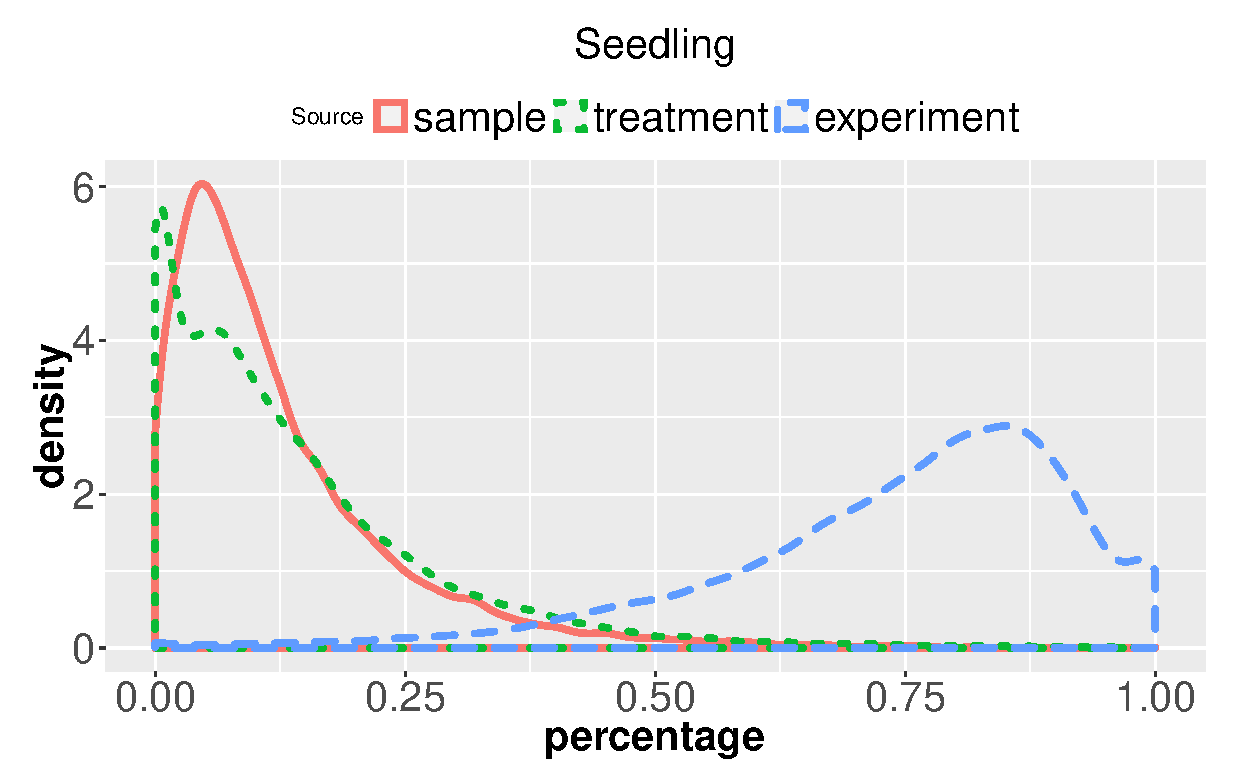
\includegraphics[scale=0.24]{../Figures/var_dens1.eps}
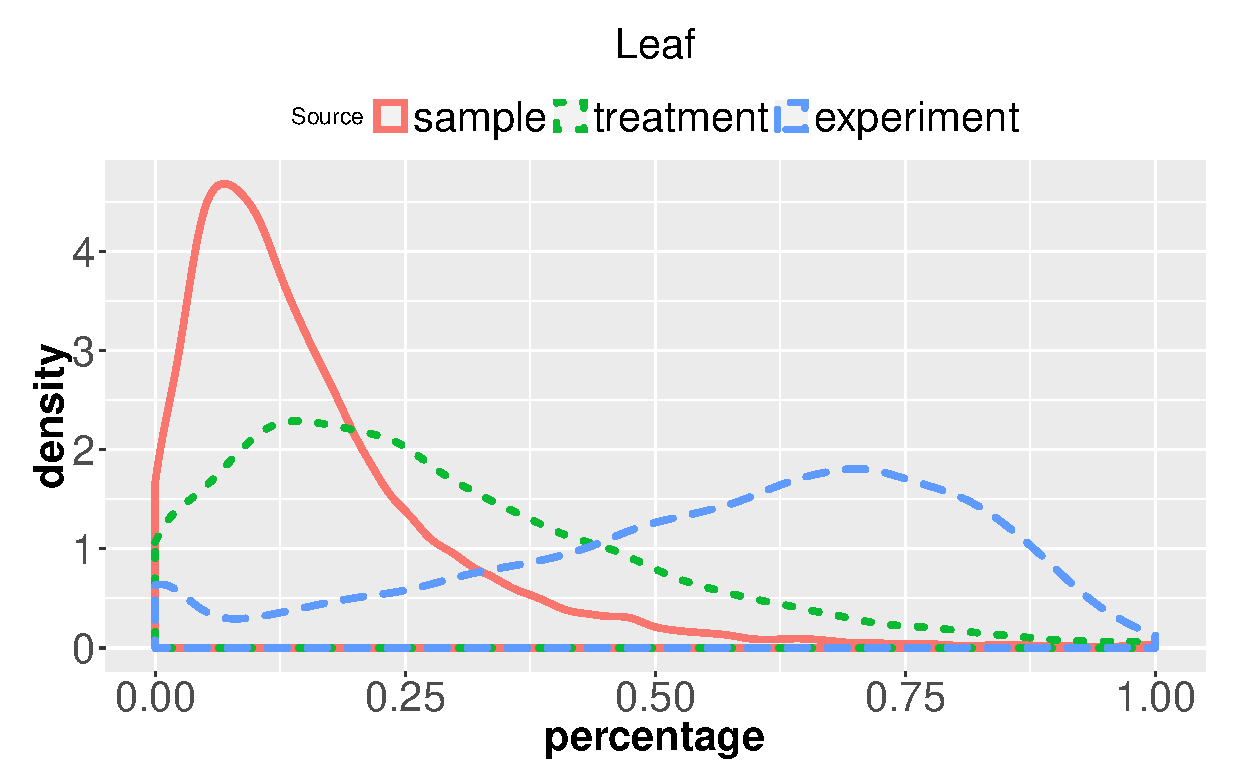
\includegraphics[scale=0.24]{../Figures/var_dens2.eps}
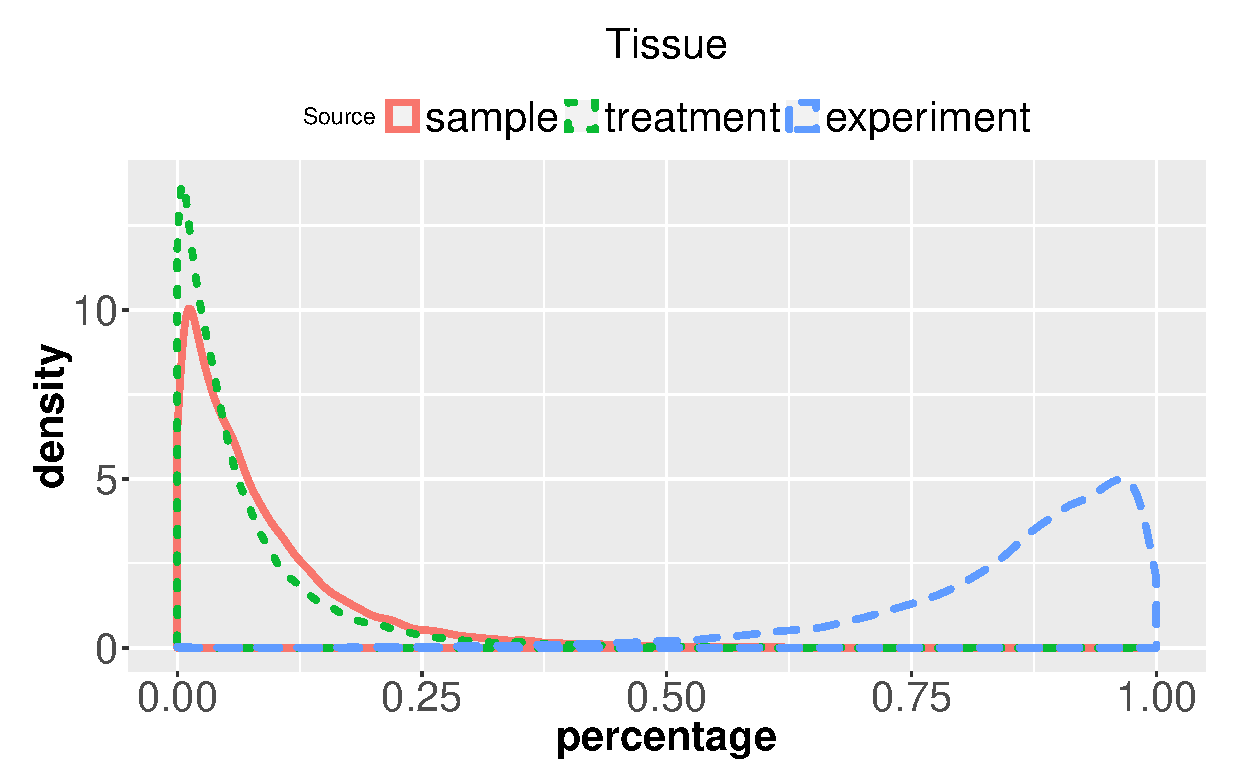
\includegraphics[scale=0.24]{../Figures/var_dens3.eps}
\end{center}
\end{figure} 


 \begin{figure}[h]
\begin{center}
\caption{\label{scatterplot} source of variation. Which one should I keep}
\includegraphics[scale=0.3]{../Figures/v1.png}
\includegraphics[scale=0.3]{../Figures/v2.png}
\includegraphics[scale=0.3]{../Figures/v3.png}
\end{center}
\end{figure} 

  \subsection{Stably Expressed Genes}
For each of the three sets, we listed top 100 genes that are identified as most stably expressed (see supplementary material for detail). Figure \ref{expressinlevel} shows the normalized CPM (counts per million,read counts devided by the corresponding library sizes and then multiplied by $10^6$, i.e. $=Y_{ij}/N_j\cdot 10^6$.  See \cite{anders2013count}) of top 5 stably expressed genes for Set 1, Set 2, and Set 3. As a comparison, we also present five traditional reference genes and five novel stably expressed genes (Figure 1) claimed in  \cite{czechowski2005genome} . We confirmed their conclusions that traditional reference genes are not necessarily stable ones (left column of Figure \ref{expressinlevel}); also, novel reference genes they suggested are relatively more stable in terms of expression level, yet not all of them are good candidates according to our results (middle column of Figure \ref{expressinlevel}). The right column displays example of 5 stably expressed genes for each set through our analysis.

\begin{landscape}
 \begin{figure}[H]
\begin{center}
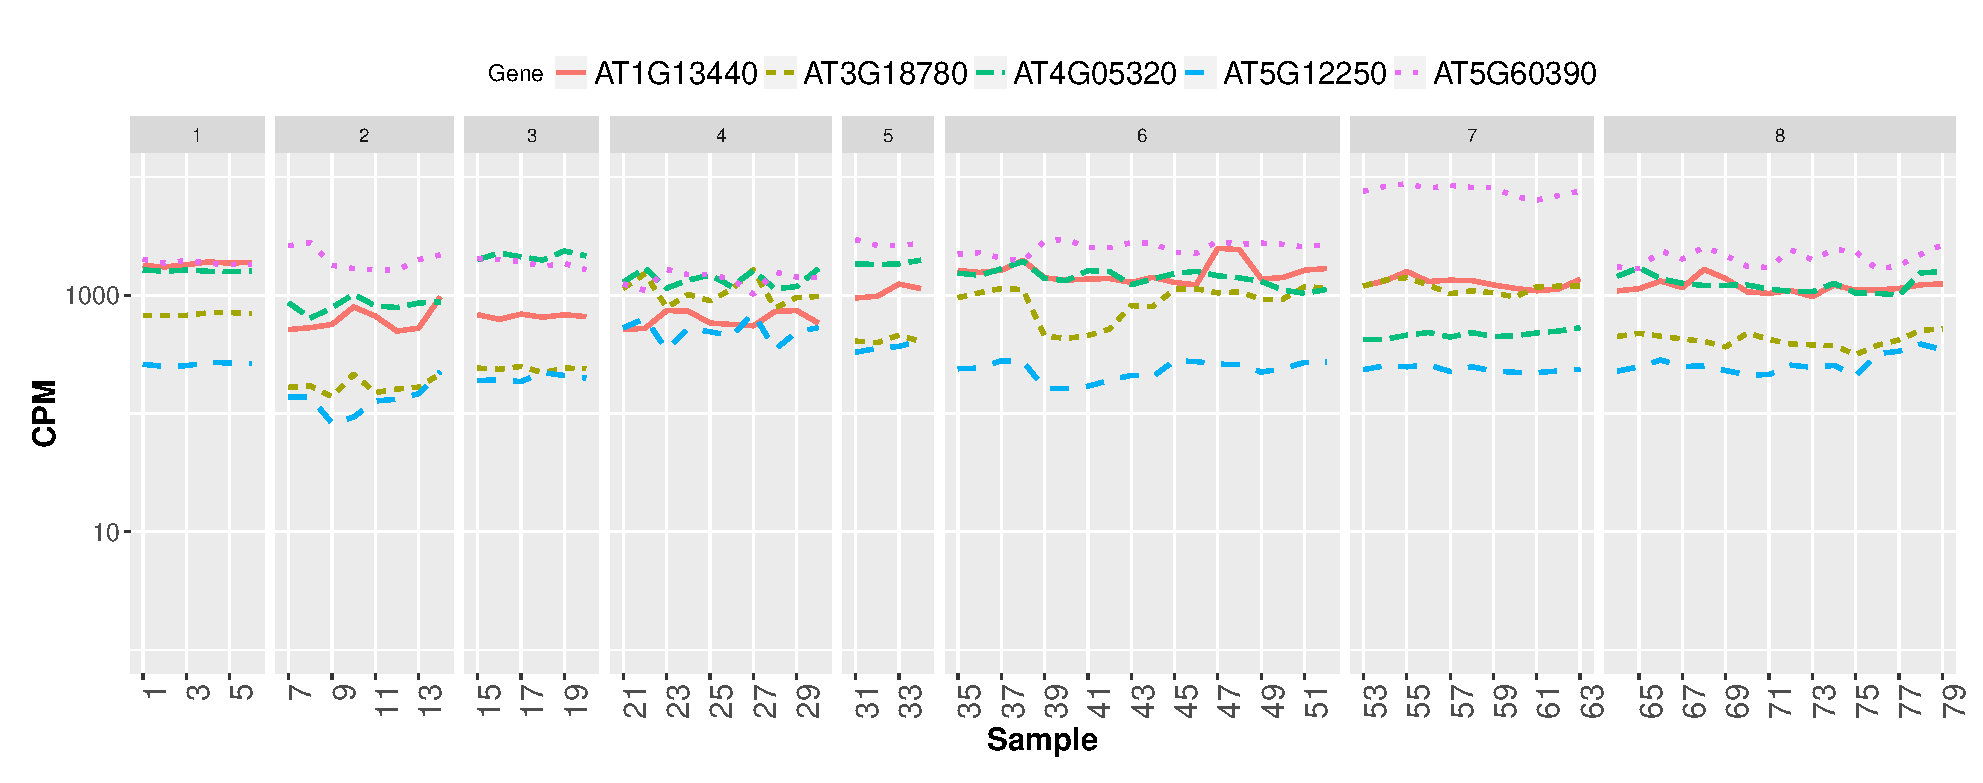
\includegraphics[scale=0.4]{../Figures/A1.eps}
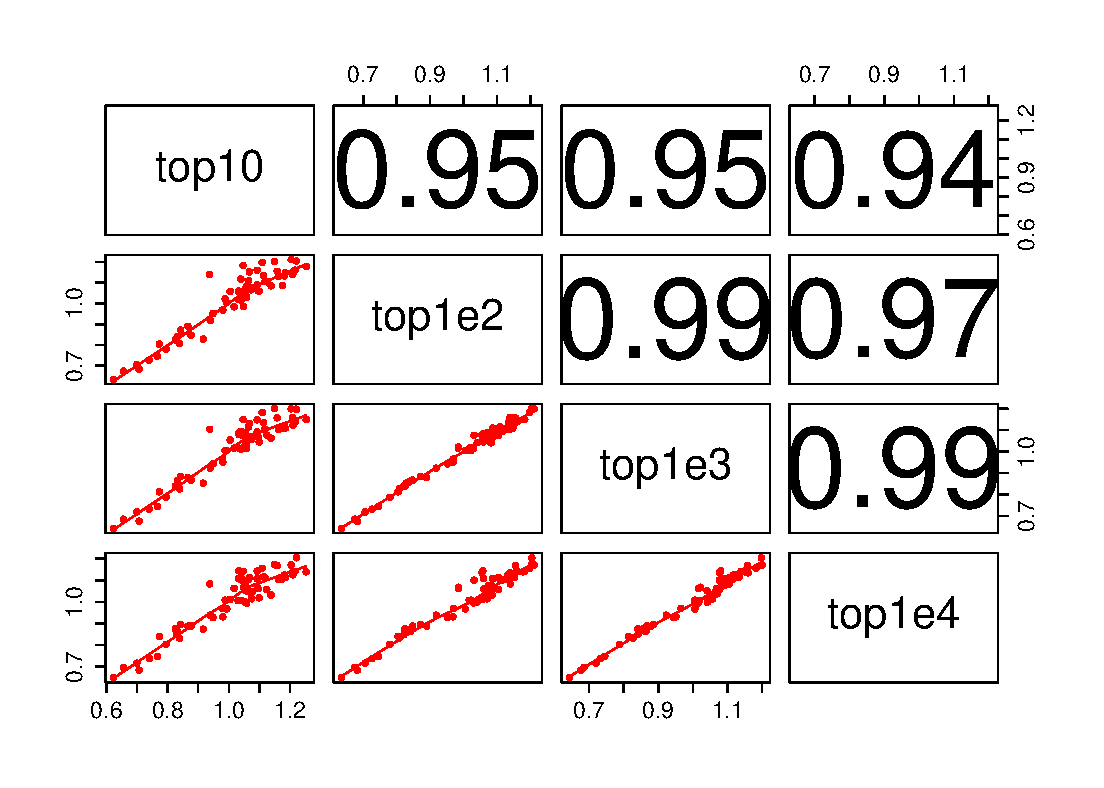
\includegraphics[scale=0.4]{../Figures/B1.eps}
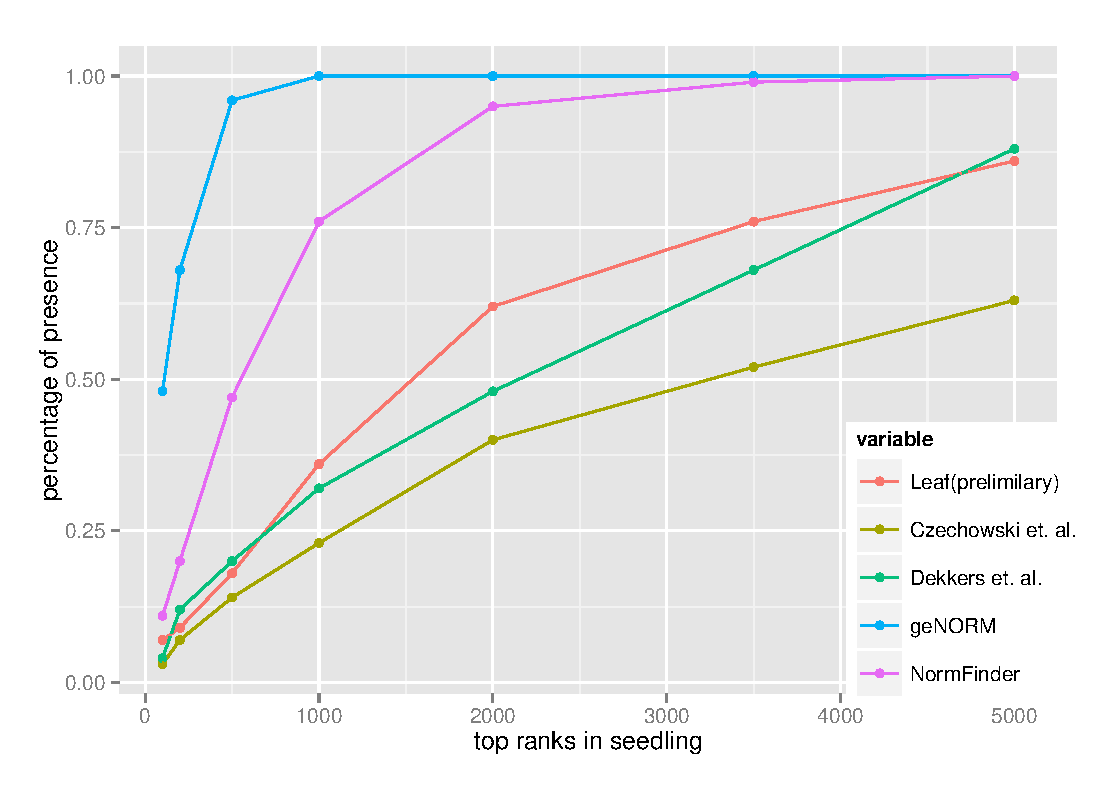
\includegraphics[scale=0.4]{../Figures/C1.eps}

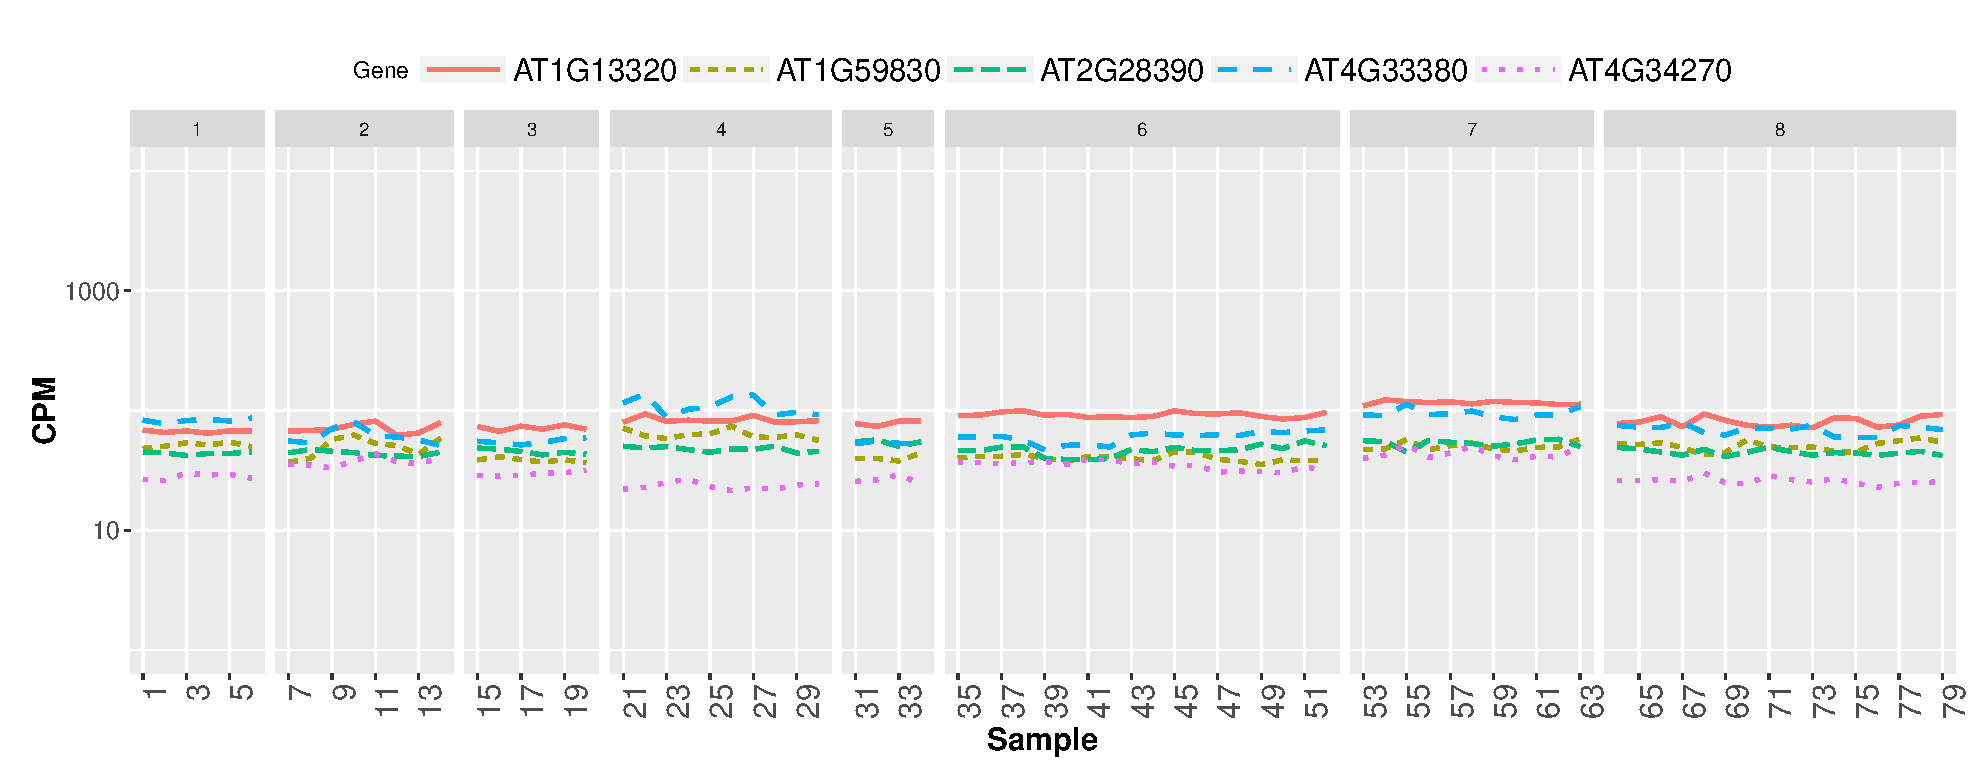
\includegraphics[scale=0.4]{../Figures/A2.eps}
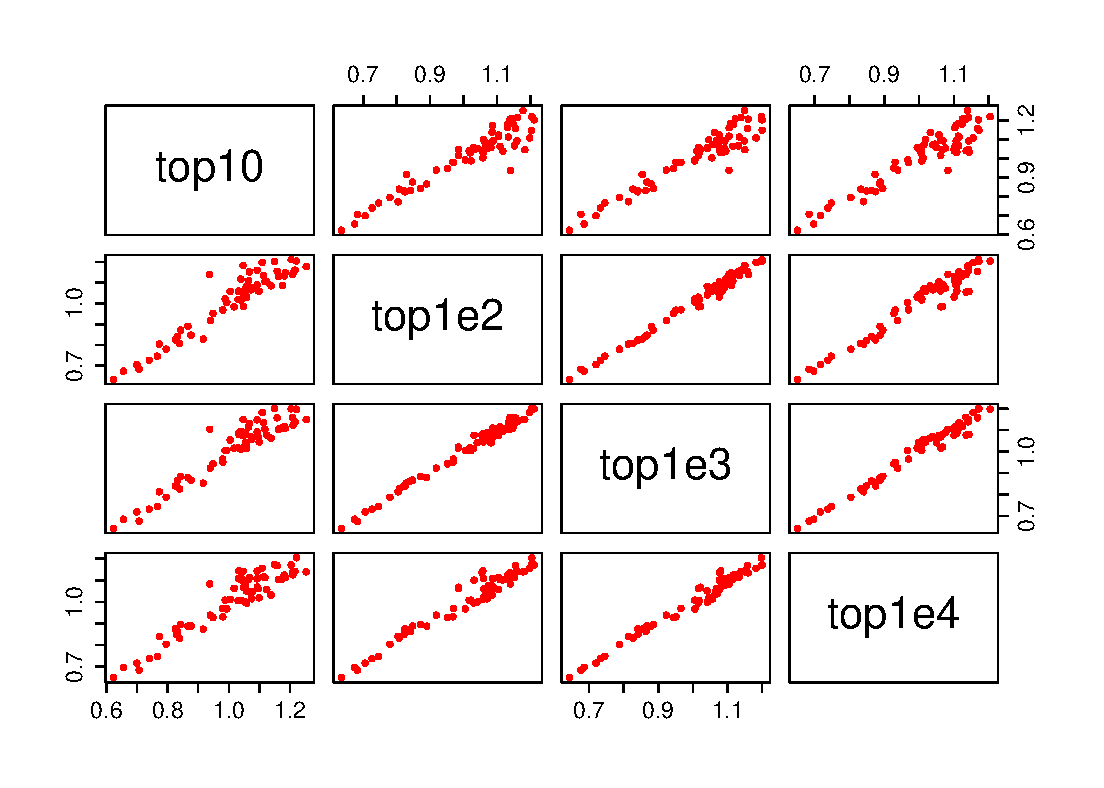
\includegraphics[scale=0.4]{../Figures/B2.eps}
\includegraphics[scale=0.4]{../Figures/C2.eps}

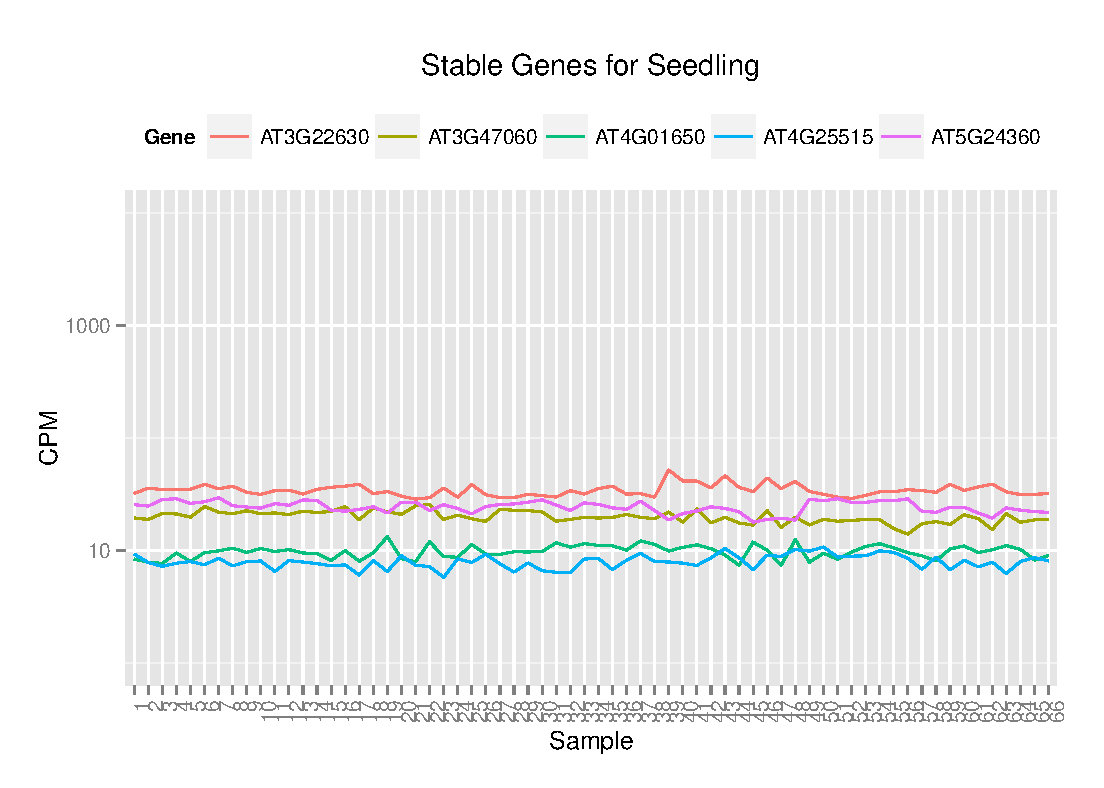
\includegraphics[scale=0.4]{../Figures/A3.eps}
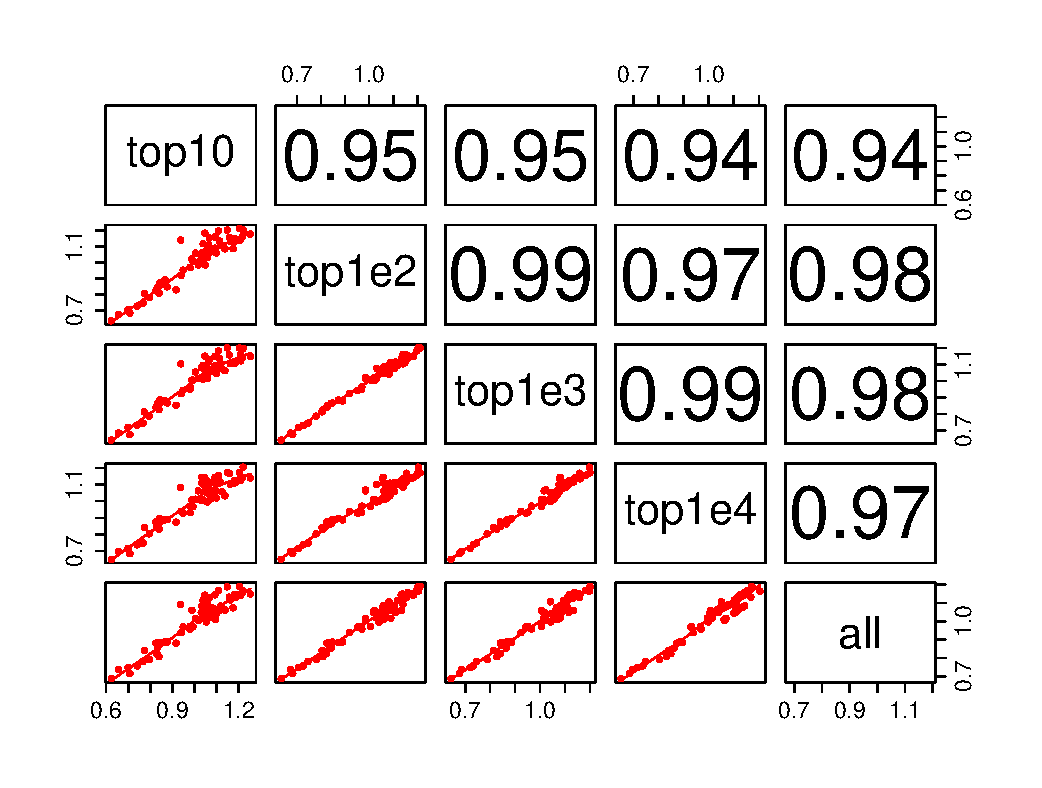
\includegraphics[scale=0.4]{../Figures/B3.eps}
\includegraphics[scale=0.4]{../Figures/C3.eps}
\caption{{\small{\label{expressinlevel} RNA-Seq expression levels of traditional reference genes in set 1(A), set 2 (D) and set 3 (G)}; expression levels of 5 stably expressed genes by \cite{czechowski2005genome}, RNA-Seq data set 1 (B), set 2 (E), and set 3 (H); expression levels of top 5 stably expressed genes identified by GLMM, RNA-Seq data set 1 (C), set 2 (F), and set 3 (I) }}
\end{center}
\end{figure} 
\end{landscape}
Figure \ref{stablegenerank} shows the relative ranks of top 100 stable genes (developmental series) from Czechowski et al., and 50 stable genes (Arabidopsis thaliana seed) from Dekkers et al. Of the 100 genes in  Czechowski, 88 are present in Set 1 we analyzed (89 for Set 2, and 88  Set 3, respectively). We found that around 30\% of them are in our top 1000 list (29 for Set 1, 31 for Set 2 and 27 for Set 3, respectively), and about 85\% are in top 5000 list (70, 77, 76 correspondingly).  On the contrast, the list of reference genes suggested by Dekkers are slightly less consistent with our list (see table \ref{table:stablegenerank} for detail). To test the statistical significance, let $N$ be the total number of genes considered, $K$ the number of genes in reference list (the list from Czechowski or Dekkers), $n$ the number of top stably expressed genes we identified,  and $X$, the number of genes confirmed as stably expressed .  We know that $X$ follows a hypergeometric distribution $P(X = k) = {K \choose k}{N-K \choose n-k}/{N\choose n}$. It is hard to calculate the exact p value due to large value of $N$. The simulated $p$ values are all 0 for the three situations for a given number of $n$. 

\begin{table}[h]
\caption{Number of genes and their percentages in top list of our analysis}
\label{table:stablegenerank}
\begin{tabular}{lrrrr r rrrr} \hline
 & \multicolumn{4}{c}{Czechowski (developmental series)} & & \multicolumn{4}{c}{Dekkers (seed)} \\ \cmidrule(r){2-10}
Top   &   100  & 500     & 1000     & 5000  &  & 100    & 500    & 1000    & 5000    \\ \hline
Set 1 &  5(5.7\%)   & 16(18.2\%)  & 29(33.0\%)  &70(79.5\%)  & &2(4\%)  &  4(8\%)  &10(20\%) & 38(76\%)   \\
Set 2 & 4(4.5\%)    &17(19.1\%)   & 31(34.8\%)  &77(86.5\%) & &2(4\%)  &  4(8\%)  &10(20\%) & 38(76\%)   \\
Set 3 &4(4.6\%)     &17(19.3\%)   &27(30.7\%)   &76(86.4\%) &  &1(2\%) & 9(18\%) &15(30\%)  & 42(84\%) \\ \hline 
\end{tabular}
\end{table}

 \begin{figure}[h!]
\begin{center}
\includegraphics[scale=0.4]{../Figures/crez1.eps}
\includegraphics[scale=0.4]{../Figures/dekker1.eps}
\includegraphics[scale=0.4]{../Figures/crez2.eps}
\includegraphics[scale=0.4]{../Figures/dekker2.eps}
\includegraphics[scale=0.4]{../Figures/crez3.eps}
\includegraphics[scale=0.4]{../Figures/dekker3.eps}
\caption{\label{stablegenerank} rank of top 100 stably expressed genes identified by Czechowski in Set 1 (A), Set 2 (B), Set 3 (C); rank of top 50 stably expressed genes identified by Dekkers in Set 1(D), Set 2 (E), Set 3 (F).  }
\end{center}
\end{figure}

Next, we explored the consistency between stably expressed genes identified from the three sets. Note that experimental data are from different labs except only 1 lab with a sample size of 6 was overlapped between Set 2 and Set 3. Our observation is that stably expressed genes are slightly more consistent within RNA-Seq data than between RNA-Seq and microarray data.  The overlaps for top ranked stably expressed genes are significantly larger, as shown in Figure \ref{fig:rankVSrank} \textbf{Need description}. Supplementary figure \ref{fig:rankAgainstrank} present rank-rank plot of Set 1 versus Set 2 and Set 1 versus Set 3.  

 \begin{figure}[h!]
\begin{center}
\includegraphics[scale=0.4]{../Figures/rankVSrank_RNA.eps}
\caption{\label{rankVSrank_RNA} This plot shows the percentage of top 100 genes in one set  in another set. Specifically, ''Tissue VS Seedling" means that, of the top 100 stable tissue genes, the pecentage of presence in top stable seedling genes.}
\end{center}
\end{figure}


\subsection{Normalization}
One particular goal of this work is to find reference genes for normalization. As a justification, we used stably expressed genes to see how normalization factors vary by choosing different lists of reference genes.   In a series of evaluations, we chose top 10, 100, 1000, 10000 stably expressed genes as reference genes, and then calculated normalization factors \citep{anders2010differential}(AH2010) for each sample in Set 1, Set 2 and Set 3. It can be seen from Figure 4 that normalization factors are more consistent when choosing 100, 1000, or 10000 reference genes in all 3 scenarios. 

 \begin{figure}[h!]
\begin{center}
\includegraphics[scale=0.3]{../Figures/norm1_u.eps}
\includegraphics[scale=0.3]{../Figures/norm2_u.eps}
\includegraphics[scale=0.3]{../Figures/norm3_u.eps}

\caption{\label{fig:scaled_diss} matrix plot of normalization factors by choosing top 10, 100, 1000, 10000 stably expressed genes for Set 1 (A), Set 2 (B), and Set 3 (C). }
\end{center}
\end{figure}

 \begin{figure}[h!]
\begin{center}
\includegraphics[scale=0.3]{../Figures/r3.eps}
\caption{\label{fig:scaled_diss} normalization factors of seedling data with stable genes from tissue }
\end{center}
\end{figure}

  \section{Discussion}
  
  
  
  \subsection{Data Process}
  A big challenge of this project is to obtain the read counts we needed. Firstly, we have limited read counts directly available in NCBI, and more importantly,  the comparability of existing count data is not validated. Those data were processed differently either in terms of software used, or versions of the same software. Both types of difference would likely introduce bias to the read counts. To avoid these concerns and to collect more data, we decided to process raw fastq file with a unified pipeline. Secondly, converting fastq format (up to 10 gigabytes per sample)  into read-count format is computationally intensive, making it essential to select adequate aligner. Two aligners were tested and compared: the standard pipeline in \cite{anders2013count} andSubread in \cite{liao2013subread}.  Our experiment shows that:  in terms of accuracy, the two procedures are comparable to each other; however, in terms of efficiency, the latter is at least three times as fast as the former. As a result, we used Rsubread to process all samples in this paper.

To assure comparability between data sets, we pre-screened experiments by several conditions. We investigated all the Arabidopsis experiments available at NCBI up to August 31, 2014. First, we only targeted on those that have biological replicates under exactly the same condition. Second, we selected experiments whose library layout were single-end. Third, we randomly chose one time period if there were repeated measurements over time, or one run if there were multiple runs. Fourth, we chose experiments with DESeq normalization factors ranging from 0.75-1.25 after we had all the read counts. 

  \subsection{Alternative method:  delete it?}
Another widely adopted approach of fitting GLMM to the data is via negative binomial (NB) regression. In many cases,  RNA-Seq data analysis begins with the assumption that $Y_{jkl}$ follows a negative binomial distribution (a.k.a Poisson-Gamma mixture) which introduces a dispersion parameter to capture the extra-Poisson variation.  In the negative binomial regression, we tried to estimate between experiment and between treatment variation. Specifically,  for each gene, we assume $Y_{jkl}\sim NB(\mu_{jkl}, \phi)$ with the link function
 \[\log(\mu_{jkl})= \xi + \log(R_{jkl}N_{jkl}) + \alpha_l + \beta_{k(l)}\]
where similarly, $\alpha_l$ is the random effect for experiment, and $\beta_{k(l)}$ is random treatment effect nested in experiments.  The only difference is that the dispersion $\phi$, rather than variance of biological sample in Poisson regression, is estimated in NB setting. We saw no significant difference in estimating the variance components between these two approaches. The NB regression is done by \verb"glmer.nb()" in \verb"lme4" package\citep{bates2012lme4} and \verb"glmmadmb()" in \verb"glmmADMB" package\citep{bolker2012getting}. Unfortunately, both implementations of NB regression experienced convergence failure. \\

A limitation of this study is that the inherent design structures are not taken into account unless when the experiment is a case-control (single factor) study. Our concern is two fold: one, although we collected more than 150 samples, they are far from enough for a complicated design structure because usually there are only 2 or 3 replicates within each treatment;  two, no available package allows for such designs under generalized linear mixed model.  In practice, if there is more than 1 factors in the experiment, we just treat it as single-factor and multiple-level. 


\section{Normalization}

Although the ability of DE detection between samples is associated with transcript length\citep{oshlack2009transcript}, \cite{bullard2010evaluation} demonstrated that the choice of normalization has the greatest impact. Previous study showed that \textit{between-sample} effects, e.g., sequencing depths, flow-cell/library preparation effects (\cite{bullard2010evaluation}, \cite{robinson2010scaling}), as well as \textit{gene-specific} effects, e.g.,  gene length or GC-contents (\cite{risso2011gc}, \cite{hansen2012removing}) are nuisance effects that may have implications on normalization, and therefore on inference of expression level and subsequent (Gene Ontology) analysis.  \\


\subsection{Biological interpretation???}
% \subsection{About the result}
%  We compared our results with earlier literature, and found our list of stably expressed genes are significantly diffenrent from previous works in microarray experiments. For the top 200 SEGs we identified from different tissues of arabidopsis, only 5 are present in Czechowski paper(2005) where they listed 100 SEGs under various conditions, and 3 are presented in Dekkers (2012) where a list of 50 SEGs were obtained by analysis of arabidopsis seed data. It is worth noting that these two sets of genes have only 3 in common. \\
%  
%  The discrepency may be due to the difference between microarray and RNA-Seq technologies.  Technical issues inherent to microarray probe performance, such as cross-hybridization and limited detection range of individual probes might contribute to contamination of data quality.  Alternative explanation of such discrepency might be limited source of RNA-Seq data, which prevented us from doing a more exhaustive research. 
%  

\section{Supplementary Material}
The details of experimental data is summarized as below

\subsection{Set 1}
\begin{landscape}
\begin{table}
\footnotesize
\centering
\begin{tabular}{p{2cm}p{2cm}p{1cm}p{4cm}p{2.4cm}p{3cm}p{4cm}} \hline
GEO Number &Tissue cluster & sample Size & Description & Age  &Col Name & Platform\\ \hline
GSE37159 &seedling &8	& Col-0, bzr1-1D, pifq and pifq;bzr1-1D  grown on BRZ-containing medium in the dark & 5 days &GSM912634-GSM912641 & Illumina HiSeq 2000\\  \hdashline
GSE38879 &seedling &12 & Transgenic line rve8-1 RVE8::RVE8:GR and rve8-1 treated with DEX or mock with three biological replicates each, 12 samples in total & 7 days  &GSM951349-GSM951360  &Illumina HiSeq 2000\\ \hdashline
GSE43865 &seedling & 6  & wild-type and link1link2 mutant plants were grown for two weeks under continuous white light conditions at 22 degrees centigrades & 9 days & GSM1072464-GSM1072469 &Illumina Genome Analyzer IIx  \\	\hdashline
GSE48767 &seedling & 6 &The wild-type seedlings and the phyA-1 mutant were grown, within each 3 biological replicates available & 4 days   &GSM1184353-GSM1184358, GSM1401633-GSM1401638 &Illumina HiSeq 2000 \\ \hdashline
GSE51119 &seedling  & 10  & homozygous ibh1(SALK 049177), ibl1(SALK 119457), 35Spro:IBH1-GFP and 35Spro:IBL1-GFP were compared to wild type (Col) &10 days  & GSM1239079-GSM1239088 &Illumina HiSeq 2000 \\ \hdashline
GSE51772 &seedling  & 8  & Col-0 and iaa3 were grown on medium for 5 days and treated with mock or 100 nMBL for 4 hr &5 days  & GSM1252262-GSM1252269 &Illumina HiSeq 2000 \\ \hdashline
GSE53078 &seedling &4 & Compare the transcriptome of HBI1-Ox and wild type & 5 days &   GSM1281703-GSM1281706 &Illumina Genome Analyzer \\ \hdashline
GSE57086 &seedling & 6  & cR-grown WT and hid1, three biological replicates for each group & 5 days &GSM1390693-GSM1390698 &GPL13222 \\ \hdashline
GSE58082 &seedling &6  &GFP-FHY1 fhy1-1 transgenic,  fhy1-1 mutant  were grown under the same light conditions used (D4d+FR3h)& 4 days &GSM1400495-GSM1400500 & GPL13222 \\ \hdashline
\end{tabular} 
\end{table}
\end{landscape}


\begin{landscape}
\subsection{Set 2}
\begin{table}
\footnotesize
\centering
\begin{tabular}{p{2cm}p{3cm}p{1cm}p{4cm}p{2.4cm}p{3cm}p{4cm}} \hline
GEO Number &Tissue cluster & sample Size & Description & Age  &Col Name & Platform\\ \hline
 GSE35288 &flower &6  & 3 biological replicates of Col-0 wild type and 3 biological replicates of the hae-3 hsl2-3 double mutant &  stage 15  &SRR401413-SRR401430 &Illumina HiSeq 2000 \\ \hdashline
GSE35408 &Hypocotyl & 10 &bzr1-1D and WT were grown in media containing 1uM PAC and 0 or 2uM PPZ for 4.5 days in dark, then treated with 10uM GA3 or mock solution for 12 hr & 4.5 days  & GSM867674-GSM867678, GSM951964-GSM951968  & Illumina HiSeq 2000 \\ \hdashline
GSE48235 &rosette leaves & 6  & For each condition (water, S1, and S3) the transcriptome was sequenced for two replicates & 9 days & GSM1072464-GSM1072469  &Illumina Genome Analyzer II \\	\hdashline
GSE53952 &seed   & 9 	& Three lines of Arabidopsis, fae1/CL37/PDAT were generated & 7-12 days & GSM1303953-GSM1303979 &Illumina Genome Analyzer IIx etc.. \\  \hdashline
GSE56326 &carpels (15 developing inflorescences) & 8 &Expression profile comparation of wild type, nga mutant and NGA overex- pression &stage 8-13&  & 	Illumina HiSeq 2000 \\ \hdashline
\end{tabular} 
\end{table}
\end{landscape}
\begin{landscape}
\subsection{Set 3}
\begin{table}
\footnotesize
\centering
\begin{tabular}{p{2cm}p{3cm}p{1cm}p{4cm}p{2.4cm}p{3cm}p{4cm}} \hline
GEO Number &Tissue cluster & sample Size & Description & Age  &Col Name & Platform\\ \hline
GSE36626 &leaves & 4 &Analysis of 2 different histone H3 variants and transcriptome in 2 conditions.  & 4 weeks &GSM897684-GSM897687 & Illumina Genome Analyzer IIx \\ \hdashline
GSE39463 &leaves  &12		&Columbia-0 pen2-1 pad4-1 sag101-2 mutant, and samples were collected at 24 hours post inoculation (hpi) of Bgh & & &Illumina HiSeq 2000 \\ \hdashline
GSE48235 &leaves & 6  & For each condition (water, S1, and S3) the transcriptome was sequenced for two replicates & 9 days & GSM1072464-GSM1072469  &Illumina Genome Analyzer II \\	\hdashline
GSE51304 &leaves  & 18 &Bisulfite-seq data for cmt2-7 single mutants, cmt3 single mutants, drm1/2 double mutants, drm1/2 cmt3 triple mutants are collected  & 3 weeks & GSM1242374-GSM1242391 &GPL13222 \\ \hdashline
GSE54677 & leaves   &20  &Col morc1 morc2 morc6 and their double mutants. For each sample, two biological replicates were performed &adult & GSM1321694-GSM1321713	 &	GPL13222\\ \hdashline
\end{tabular} 
\end{table}
\end{landscape}


 \begin{figure}[h!]
\begin{center}
\includegraphics[scale=0.5]{../Figures/rank_sl.eps}
\includegraphics[scale=0.5]{../Figures/rank_st.eps}
\caption{\label{fig:rankAgainstrank} Rank plot of stably expressed genes,  Set 1 versus Set 2 and Set 3.}
\end{center}
\end{figure}

\newpage


\bibliographystyle{apalike}
\bibliography{mybib}

\end{document}

